\documentclass[hidelinks, 12pt, a4paper]{article}

\usepackage[utf8]{inputenc}
\usepackage[margin=1.5cm]{geometry}
\usepackage{graphicx}
\usepackage{setspace}
\usepackage[T1]{fontenc}
\usepackage{tocloft}
\usepackage{todonotes}
\usepackage{epstopdf} 
\usepackage{hyperref}
\usepackage{float}
\usepackage{titlesec}
\usepackage{listings}
\usepackage{multirow}
\usepackage{xcolor}
\usepackage{mwe}
\usepackage{hyperref}
\onehalfspacing
\usepackage[english]{babel}
\usepackage{fancyhdr}
\usepackage{enumitem}

\pagestyle{fancy}
\fancyhf{}
\rhead{blulancetech@gmail.com}
\lhead{Carpool}
\rfoot{Page \thepage}

\author{}
\date{}
\title
{
	
\includegraphics[width=6cm]{images/up_logo.jpg} \\
	Department of Computer Science \\
	Faculty of Engineering, Built Environment \& IT\\
	University of Pretoria \\
	\vspace{0.5cm}
	\Huge COS301 -
	Software Engineering\\
	\vspace{1cm}
	{\Huge Carpool}\\
	\begin{Large}
	Architectural requirements document
	\end{Large}
	\vspace{0.5cm}
	
    \begin{center}
    \noindent
    
\includegraphics[width=6cm]{images/company_logo.png} 
    \vspace{0.5cm}
    \begin{table}[h]
    \centering
    \begin{tabular}{|l|l|l|}
    \hline
    Name  & Student Number\\ \hline
    Benjamin Osmers & u16068344 \\ \hline
    Ashleigh Govender &  U20528834      \\ \hline
    Joshua Brink  & U19185678 \\ \hline
    Jason Antalis     & U19141859     \\ \hline
    Wesley Pachai & U20578688    \\ \hline
            
    \end{tabular}
    \end{table}
    \end{center}
    }

\begin{document}
\maketitle


\newpage
\tableofcontents
\newpage
\section{Architectural design strategy}
\newpage
\section{Architectural design styles}
\newpage
\section{Architectural Quality requirements}
\textbf{Usability:}
\newline
The user should be able to use the application in a way that is intuitive and easy to use.
The User Interface will be easy to understand and use.
Buttons and clear actions will be shown on the screen only.
\newline
\textbf{Scalability:}
\newline
The system should be able to handle a large number of users.
Meaning that the system should be able to handle many drivers posting rides and passengers booking rides.
As well as, the system's performance should not be reduced at peak hours.
\newline
\textbf{Availability:}
\newline
This app should be available to all users, at all times.
For example, if a driver wants to post a ride at the middle of night and a passenger wants to book a ride at the same time then the system should be able to handle this.
Hey
\newline
\textbf{Supportability:}
\newline
The driver should have a map showing the location of the passengers who have booked a ride.
The passenger should have a map showing the location of the drivers who have posted a ride.
The maps should show a route between the two locations.
\newline
\textbf{Security:}
\newline
The system should be secure when doing any form of user authentication within the app.
Meanwhile, on the database side it will also have be secure with protective administraive details.
For example: when a user signs up the password will be salted then hashed and stored in the database.
\newline
\newpage
\section{Architectural design and patterns}
\textbf{Client-server Pattern:}
\newline
The application will be used by many users and therefore the application will be used in a client-server pattern.
It will consist of drivers and passengers whom will need to connect to the server for usage.
The database will be used to store the drivers, passengers and various trips which will be posted and receive bookings for.
\begin{center}
    \noindent
    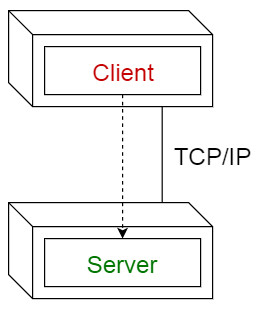
\includegraphics[width=4cm]{images/client_server.png}
    \vspace{0.5cm}
\end{center}
\textbf{Model View Controller:}
\newline
Since the app will need to query the database and update the database, the app will be used in a MVC pattern.
The app will have the layout to be like a model view controller, for example: the passanger will have to be able to view available trips (view -> controller -> model).
For the driver they will have to update the model, posting a trip in other words, to then be able to see thier trips (view -> model).
\begin{center}
    \noindent
    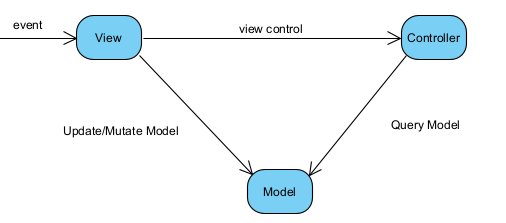
\includegraphics[width=10cm]{images/model_view_controller.png}
    \vspace{0.5cm}
\end{center}
\textbf{Layered:}
\newline
The app will be used in a layered pattern as well since a model view controller can also be thought of as multiple layers.
This pattern will be shown as a means of communicating between the backend, database and the front end.
\begin{center}
    \noindent
    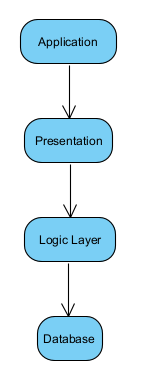
\includegraphics[width=4cm]{images/layered.png}
    \vspace{0.5cm}
\end{center}
\newpage
\section{Architectural constraints}
\newpage
\section{Technology Choices}
\end{document}